\smalltitle{سوال 3}
\\\noindent
در این قسمت از اکثر قسمت کد‌های دفعه‌ی قبل استفاده می‌کنیم. در ابتدا یک متغیر
\lr{global}
از جنس آرایه کارکتر به اسم
\lr{exchanged}
تعریف می‌کنیم. در ابتدا مقدار این متغیر
\codeword{NULL}
است. تمامی ترد‌های
$B$ تا $D$
به کمک یک
\lr{condvar}
صبر می‌کنند که ترد
$A$
به این متغیر مقدار دهد.
مقداردهی به این متغیر بدین صورت انجام می‌گیرد که در ابتدا مموری
\lr{page aligned}
به اندازه‌ی سایز فایل
\lr{allocate}
می‌کنیم. سپس به کمک
\codeword{mmap}
فایل را به مموری مپ می‌کنیم.
سپس از انجایی که دیگر
\lr{exchanged}
برابر
\codeword{NULL}
نیست، ترد‌های دیگر نیز شروع به کار می‌کنند.

در ابتدای اجرای برنامه نیز دو فایل به نام‌های
\lr{dummy1} و \lr{dummy2}
به اندازه‌ی ۴ کیلوبایت ایجاد می‌کنیم که آنها را به مموری
\lr{map}
کنیم. محتویات این فایل‌ها رندوم است.

در ابتدا برنامه را برای یک بار برای هر حالت اجرا می‌کنیم.
\begin{figure}[H]
    \centering
    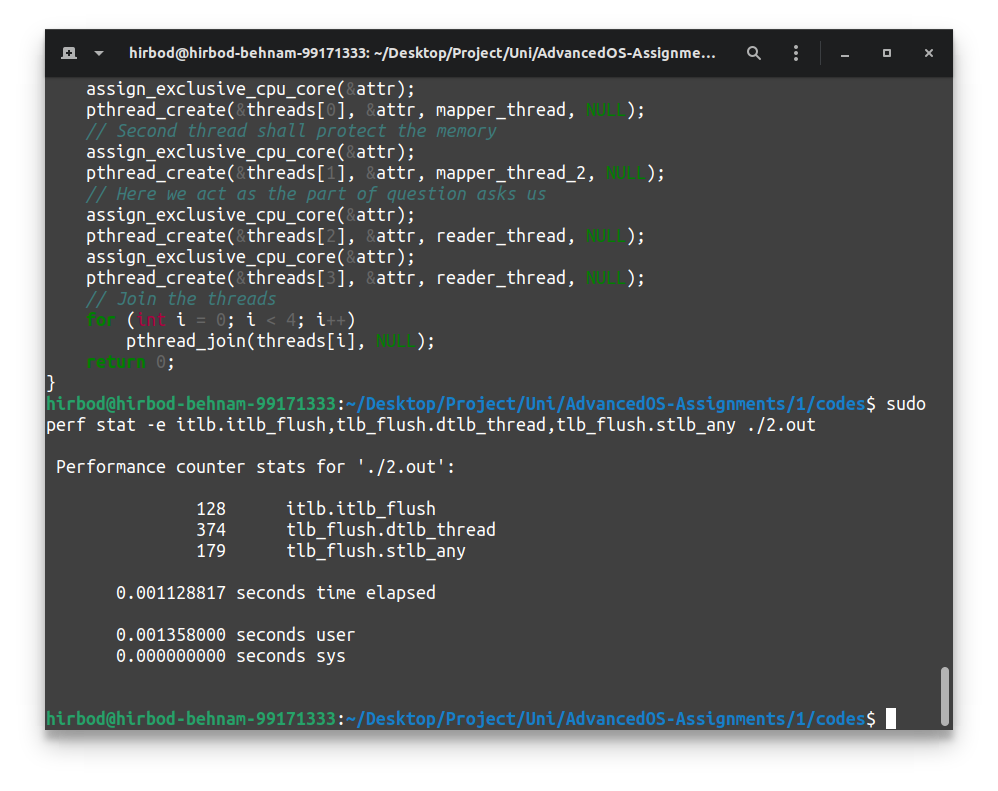
\includegraphics[scale=0.4]{pics/2-read-read.png}
    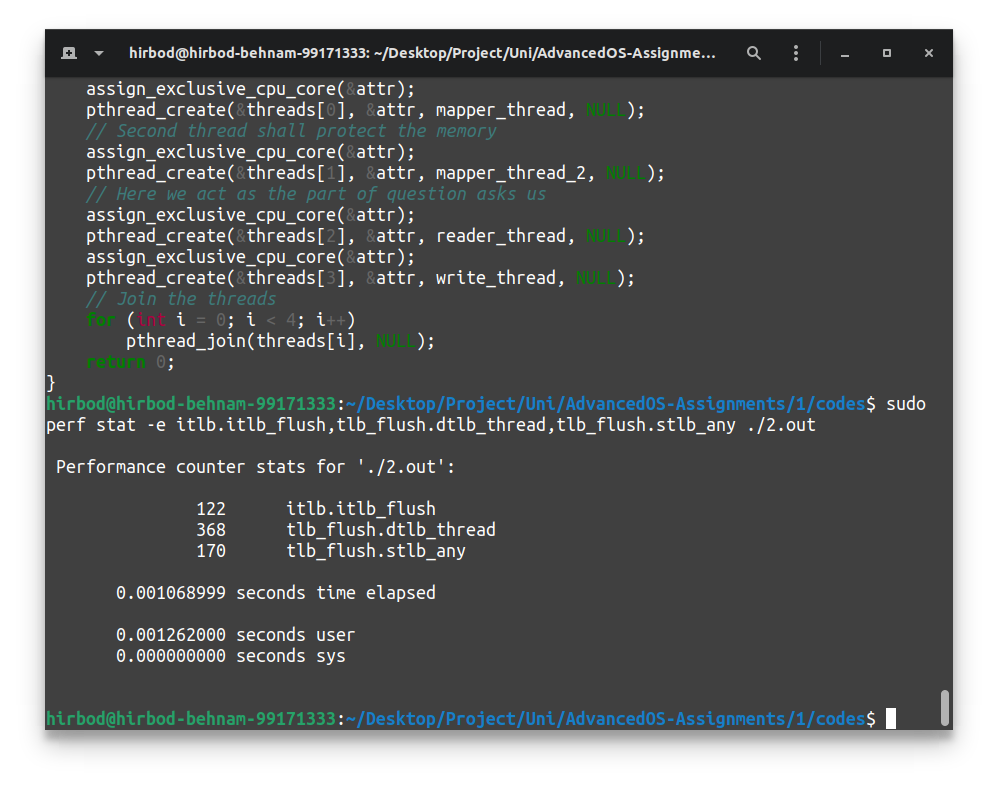
\includegraphics[scale=0.4]{pics/2-read-write.png}
\end{figure}
\begin{figure}[H]
    \centering
    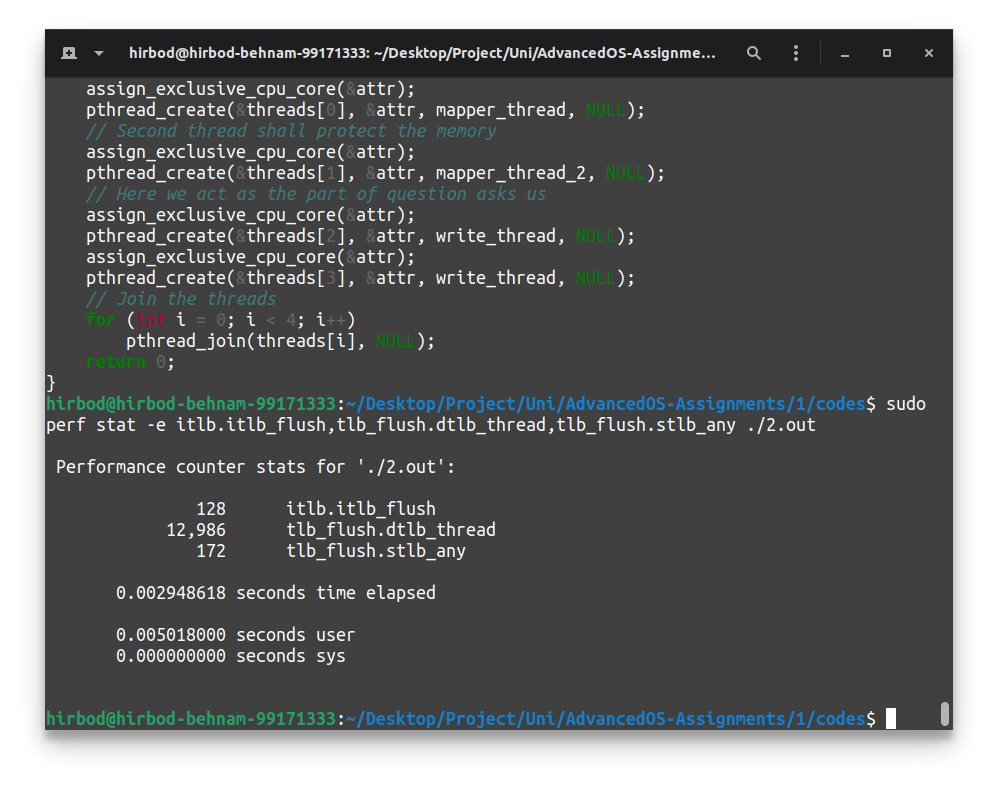
\includegraphics[scale=0.4]{pics/2-write-write.png}
\end{figure}
همچنین برای دقیق‌تر شدن نتایج من اسکریپتی نوشتم که به تعداد زیاد برنامه را اجرا می‌کند و نتایج را در
یک فایل
\lr{csv}
ذخیره می‌کند. فایل‌های خام
\lr{csv}
را در قسمت کد‌ها فرستاده‌ام ولی در این گزارش صرفا میانگین حالات را آورده‌ام.
برای اجرا کردن 
\lr{perf}
دقیقا از همان دستور سوال قبل استفاده کردم.
برای بدست آوردن میانگین نیز از دستور
\link{https://stackoverflow.com/a/18726910/4213397}{این لینک}
استفاده کردم.
\begin{latin}
    \centering
    \begin{tabular}{cccc}
    \hline
    Test & itlb & dtlb & stlb\\
    \hline
    read read & 126.851 & 358.317 & 170.248 \\
    \hline
    read write & 129.545 & 361.851 & 172.871 \\
    \hline
    write write & 132.426 & 11925.7 & 169.772 \\
    \hline
    \end{tabular}
\end{latin}
تفاوت چندانی در قسمت
\lr{itlb} و \lr{stlb}
مشاهده نمی‌شود. ولی در حالتی که دو ترد نویسنده داشته باشیم متوجه می‌شویم که مقدار
\lr{dtlb}
به‌شدت افزایش می‌یابد. من خیلی دلیلی نداشتم برای این موضوع و به خاطر همین موضوع کمی در اینترنت به دنبال جواب گشتم.
بعد از کمی جست و جو به
\link{https://news.ycombinator.com/item?id=19805675}{این صحفه}
رسیدم که کسی در آن همچین چیزی نوشته بود:
\begin{latin}
\begin{quote}
    Writable mappings are problematic though, because of the unpredictable pauses caused by the TLB shutdowns required to maintain coherence of the dirty flag. 
\end{quote}
\end{latin}
حال برای قسمت دوم سوال، کد را به صورت خواسته شده عوض می‌کنیم. در ترد دوم صرفا به کمک تابع
\codeword{munmap}
در ابتدا مموری را
\lr{unmap}
می‌کنیم و سپس به کمک
\codeword{close}
فایل را می‌بندیم. این کار باعث می‌شود که برنامه همیشه
(مگر زمانی که ترد $C$ و $D$ کارشان زودتر تمام شود)
\lr{segmentaion fault}
بخوریم چرا که دیگر مموری مشخص شده در
\lr{exchanged}
معتبر نیست. این اتفاق به دلیل
\lr{TLB shootdown}ی
می‌افتد که منشا آن ترد
$B$
و تابع
\codeword{munmap}
است.
(
    \link{https://news.ycombinator.com/item?id=19805675}{منبع 1}
    \link{https://stackoverflow.com/a/68711191/4213397}{منبع 2}
)
اسکرین‌شات‌‌های اجرای برنامه در زیر آماده است.
\begin{figure}[H]
    \centering
    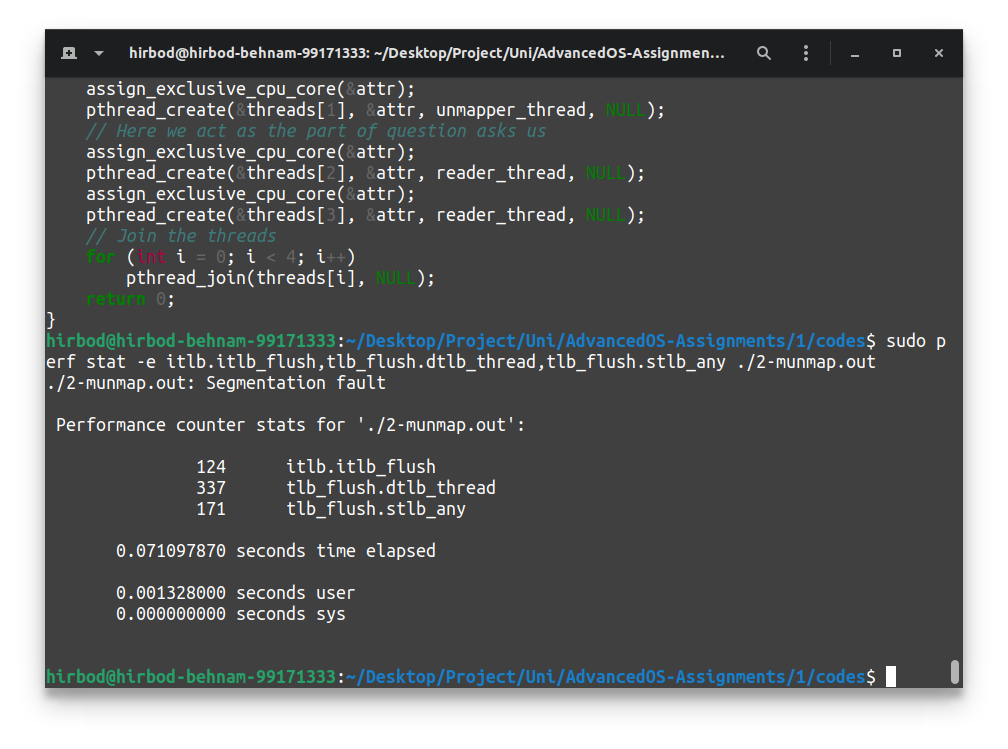
\includegraphics[scale=0.4]{pics/2-unmap-read-read.png}
    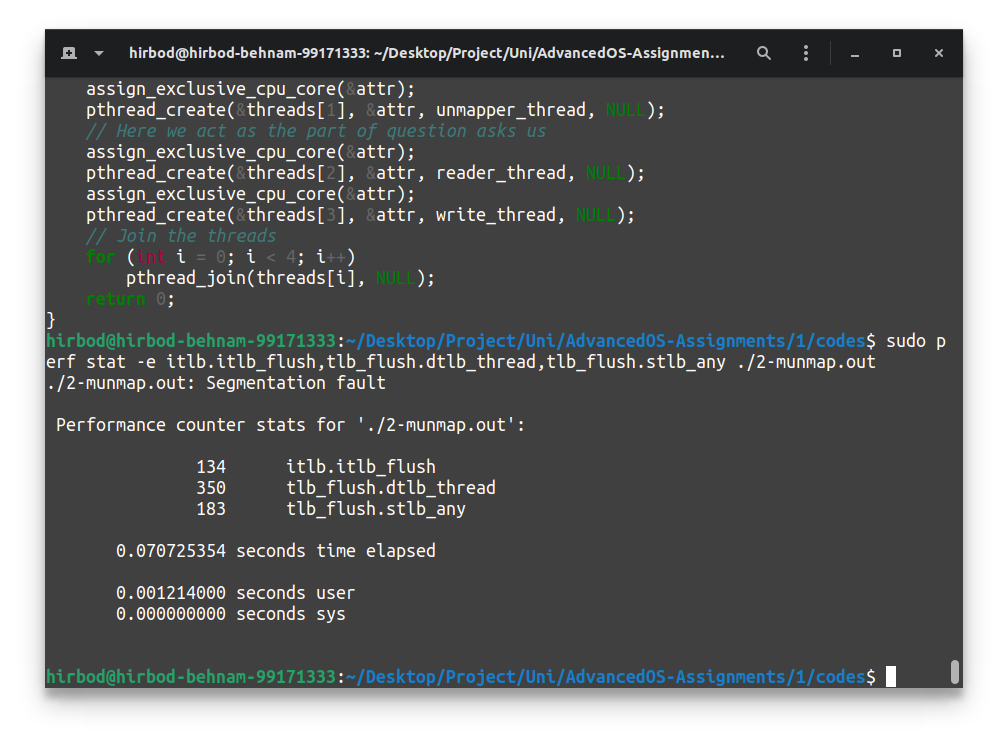
\includegraphics[scale=0.4]{pics/2-unmap-read-write.png}
\end{figure}
\begin{figure}[H]
    \centering
    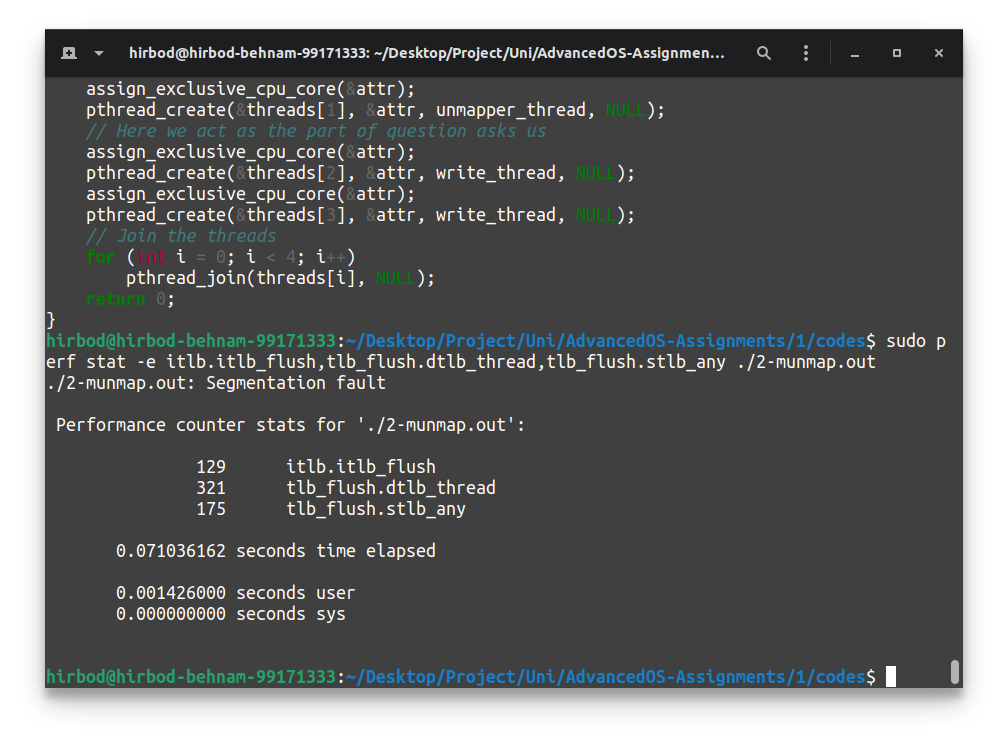
\includegraphics[scale=0.4]{pics/2-unmap-write-write.png}
\end{figure}
همان طور که مشخص است تمامی برنامه‌ها به
\lr{Segmentation fault}
بر می‌خورند.


